\documentclass[../main.tex]{subfiles}
\begin{document}

\chapter{Kraftværk} \label{Chap:Kraftværk}

\section{Generator}
Generatoren består af 2 motorer. DC motoren skal forestille at være en turbine fra et kraftværk der driver en AC generator. Generator er en asynkron 14 polet motor med en 924 rpm/V dette output bliver så forbundet til en 3 phaset transformer. Efter denne transformer bliver det forbundet til en 3 phaset full bridge rectifier. På outputtet af rectifier skal der være 15V samt den skal kunne lever 300mA. Ud fra dette kan den optimale transformer opstilling findens. DC motoren drives af et PWM signal, der kører med så høj frekvens, at det for motorens vedkommende, bliver glattet ud til en specifik spænding.

\subsection{Fuld bridge rectifier}
for at omdande det 3 fase output fra transformen til DC bruges der en Fuld bridge rectifier. samt en udglatnings kondensator dette resultere i kredsløbet 

\begin{figure}[H]
      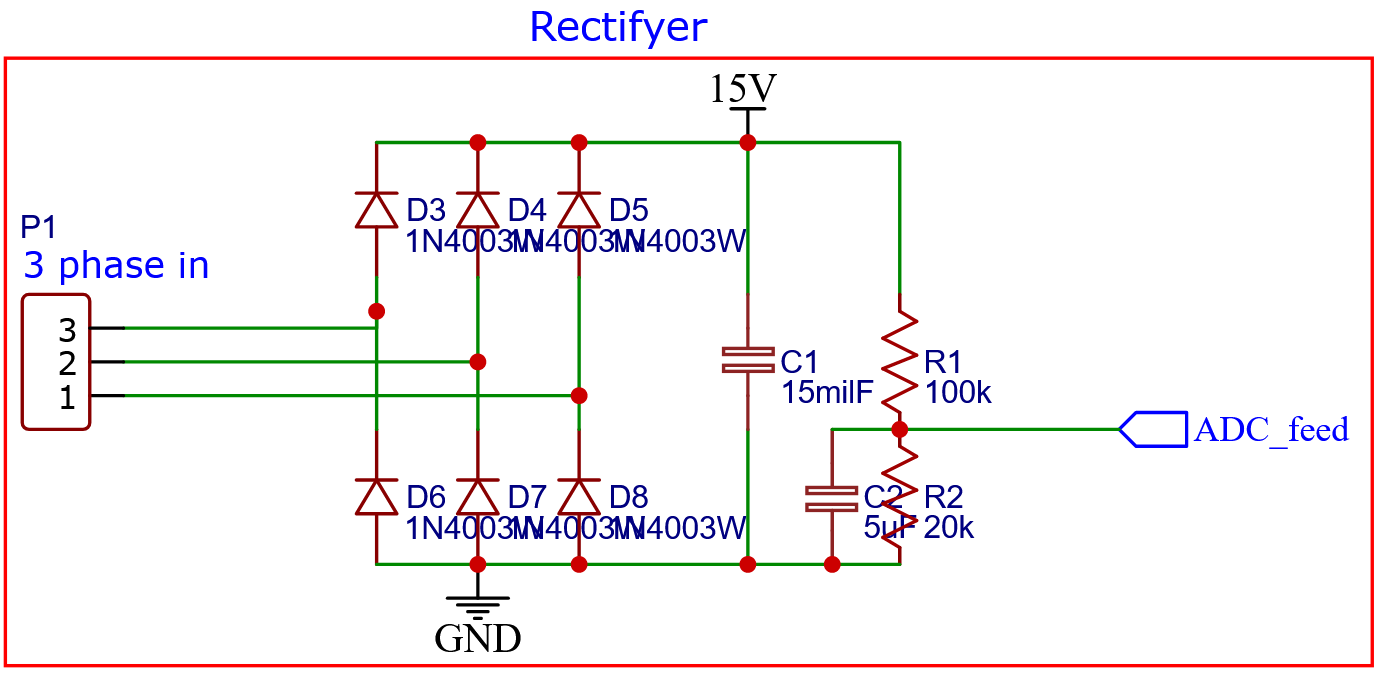
\includegraphics[width=\textwidth]{Dokumentation/Figures/Rectifyer_dig.png}
     \caption{Diagram over 3 fase Fuld bridge rectifier}
     \label{fig: Rectifyer_dig}
     \end{figure}
som det kan ses af kredsløbet er der også lavet en spændings deler med indbygget lowpass filter dette bruges til feedback til Arduino som styre Generator. og da arduinoen kun kan klare et signal mellem 0 og 5 volt. og ved  12v på DC motoren er der set op til 25V vælges en 1 til 6 spændings deler så der er 5V buffer.
for en full bridge rectifier kan DC spænding  beskrives ud fra 
$$ V_{DC} = \frac{2}{\frac{2 \cdot \pi}{6}}\int_{0}^{\frac{\pi}{6}}\sqrt{3}\cdot V_f \cdot cos(\omega t) d(\omega t) = \frac{3 \cdot \sqrt{3}}{\pi} \cdot V_f = 1.654 \cdot V_{fpp} $$
og ud fra dette kan vi finde den nødvende output spænidng fra transformerend 
$$ V_{f}= \frac{15V}{1.654} = 9.068V$$
ud fra denne information kan transformen designes.
\subsection{Transformer}
transformen består af 3 en-fasede ringkerne transformere med Omsætningsforhold 1:8. og kobling kan fridt vælges. da rectifyeren kun har brug for 9V peak per fase for at opnå 15V DC ønskes forstærning at være så lille som mugligt da generatorn har en KV på $ 924 \frac{rpm}{V}$  og dc motor har en tomgang hastighed på 5887 rpm samt vi ønsker at DC motor skal køre ved så høj en rpm som mugligt. af disse grunde vælger vi en transformer koplingen stjerne delta da denne giver den laves muglig forstærknig. eftersom den har minds muglig spænding på primære siden af transformen. samt den på sekundær siden har minds muglig fase spænding dette giver en forstærknig på
$$ V_{in} =\frac{ V_f \cdot \sqrt{3}}{\frac{N_2}{N_1}} = \frac{9.068V \cdot \sqrt{3}}{\frac{8}{1}} = 1.963V$$
$$n = \frac{V_f}{V_{in}}=4.618$$




\section{Buck Converter}
For at sikre den rigitge spænding til Energilageret, skal der implementeres en step-down/buck converter, der kan holde en output spænding på 4.8 volt med en input spænding på ca 15 volt fra generatoren. Da input spænding kan variere med op til 1 volt + og minus, er det vigtigt der indgår et feedback system så output spændingen holder den ønskede værdi og Energilagret ikke bliver overopladt.

\subsection{Opbygning}
Buck konverteren er opbygget efter et basic buck converter circuit, der består af en mosfet transistor, en Kondensator, en diode og en spole. Mosfet transistoren udgør selve ideen af buck converteren, det er den der åbner og lukker for inputtet med et bestemt duty cycle, som man ved at ændre også ændre på output spændingen. Ved at gøre dette får man også et step hver gang der bliver åbnet og lukket, også kaldet ripple, derfor bruges en kondensator som oplades og aflades hver gang transistoren henholdsvis er lukket og åben som minimere output ripple. yderligere minimere man ripple effektet med en spole, udover det bruges en spole også da den giver buck converteren en højere effektivitet, i modsætningen til feks en modstand som ville afgive termisk energi. Dioden er sat til ground lige før spolen for at sikre der kan flyde strøm igennem opsætningen også når mosfetten er åben. 
I buck konverteren ved kraftværket var der problemer med at aktivere mosfetten og få PWM signalet igennem, derfor blev der forsøgt med et driver system med en BJT transistor, hvilket gav det ønskede output. 

\subsubsection{Komponenter}
Komponenterne som er brugt til opbygningen af buck konverteren er udvalgt ved hjælp af udregninger fra ashraf minikursus, og ud fra \ref{subsection:Buck konverter}, udover de beregnede værdier er der ved hjælp af test og målinger på kredsløbet valgt nogle enten højere eller lavere værdier for at få en buck konverter som ønsket.


\subsection{Kontrollering}
For at styre Duty Cycle af PWM signalet, så converteren altid holdte 4.8V, brugte vi en Mega 2560 og samplede outputtet (som var blevet neddelt med en spændingsdeler). Derefter blev der bygget et while loop der hvert millisekund op- eller nedjusterede duty cyclen, afhængig af om ADC værdien var over eller under den ønsket værdi. Controlleren var hurtig og gjorde at Buck Converteren altid leverede 4.8V. 

\section{Styring af kraftværk}
Kraftværket skal styres så der altid leveres 15V til indgangen på Buck Converteren. Da belastningerne kan ændre sig, er det ikke nok blot at sætte en proportional gain på. Der er nødt til at designes et system med feedback, så den aktuelle spænding kan sammenlignes med den ønskede. Dette realiseres med en PI-Lead kontroller, der udarbejdes efter de metoder vi lærte i kurset \emph{34722 - Reguleringsteknik 1}.

\subsection{Modellering}
Første skridt var at modellere systemets egenskaber i Matlab. Dette blev gjort ved at lave små steps på inputtet (OCRnB værdier) og måle hvordan outputtet reagerer (ADC værdier). Vi omregnede ikke til spændinger og duty cycle, da vi dermed kunne lave færre beregninger på mikrokontrolleren. Outputtet blev målt med et oscilloskop og gemt til en CSV fil som blev importeret til Matlab. Derefter kan Matlab fitte en overføringsfunktion. Dette kan ses i nedenstående graf, hvor den grå linje er det reelle output (ADC værdier) og G er den fittet overføringsfunktion. 

\begin{figure}[H]
      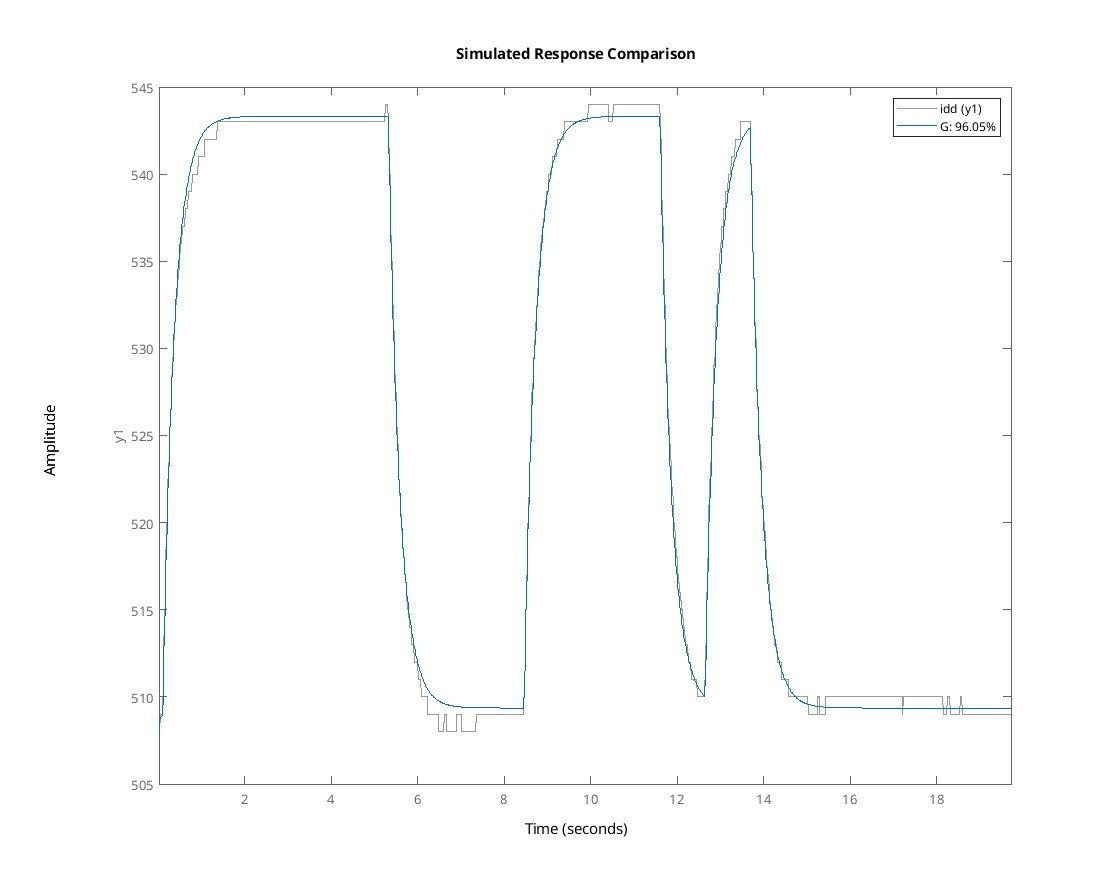
\includegraphics[width=\textwidth]{Dokumentation/Figures/Motor Model Fit.jpg}
     \caption{System Overføringsfunktion}
     \label{fig: System Overføringsfunktion}
     \end{figure}

\subsection{PI-Lead Kontroller}
Derefter kan PI-Lead kontrolleren nu designes. Vi vælger en phase margin på 60 grader, da det giver en god balance mellem hastighed og stabilitet. Vi tilpasser Ni og alpha værdierne indtil vi finder et system der hurtigt, men ikke så hurtigt at motoren ikke kan følge med. Nedenstående figur viser en step respons af systemet med PI-Lead kontroller. Der er en smule overshoot, men det gav ikke nogle stabilitetsproblemer.

\begin{figure}[H]
      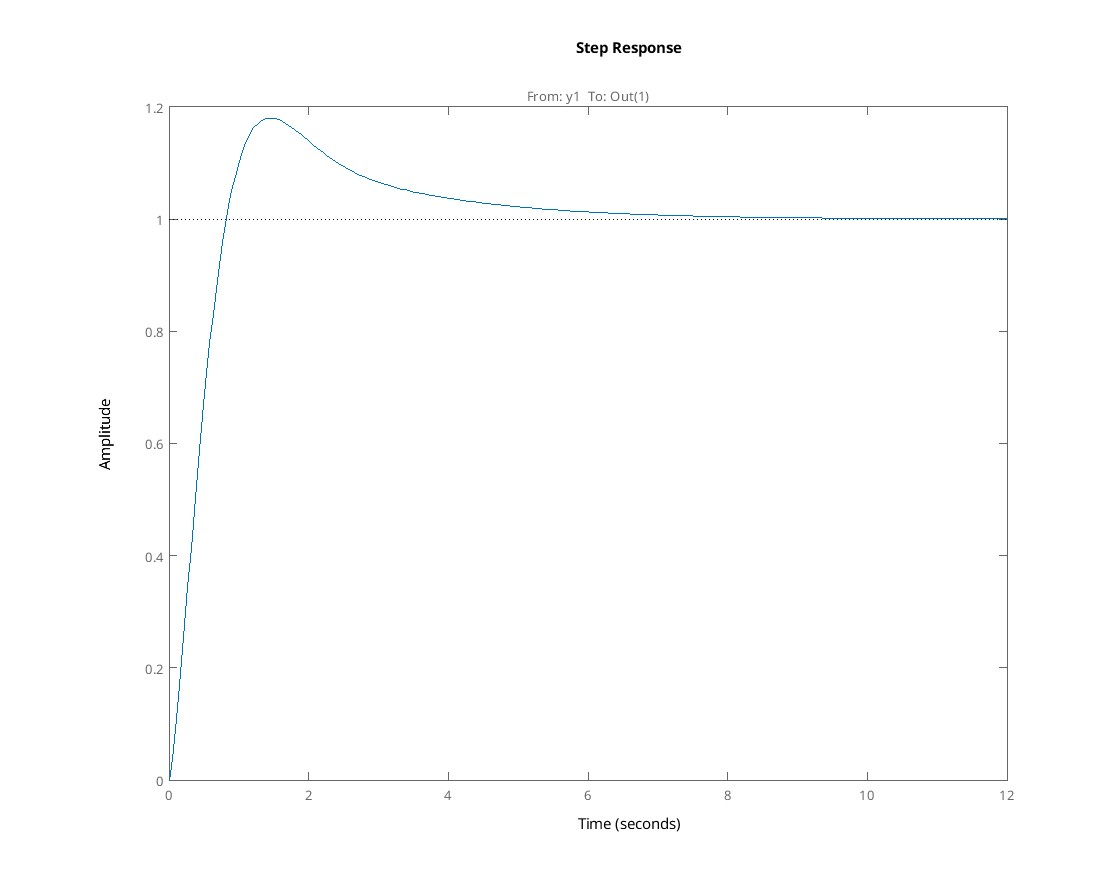
\includegraphics[width=\textwidth]{Dokumentation/Figures/Motor PID Step Response.jpg}
     \caption{System Overføringsfunktion}
     \label{fig: System Overføringsfunktion}
     \end{figure}

Nu skal denne PID kontroller, som er en overføringsfunktion i S-domænet, omdannes så den kan blive implementeret i kode. Dette gøres ved at Z transformere den med en indbygget Matlab funktion, hvor vi bruger ADC samplingsraten som input. Transformationens parametre skrives til en Data.h fil, som resten af C-koden benytter. Dette gør at vi kan iterere hurtigt og præcist. Z transformationens parametre kan nemt implementeres ved at gemme forrige inputs og outputs, og gange dem med et specifikt gain. I vores tilfælde gemmes der 2 forrige outputs og 1 forrigt input. Derefter ganges hvert input/output med deres tilhørende parameterværdi og alle værdierne lægges sammen. Dette outputtes som OCRnB værdi, der benyttes af PWM timeren.

\subsection{PWM Driver}
Da Arduino Mega'en maksimalt kan levere 40mA far et enkelt output, skal der designes et driver kredsløb, der skalerer Arduinoens signal til en markant større strøm (+2A i nogle tilfælde). Dette gøres ved brug af en IRF530N power MOSFET. Figur \ref{fig: PWM Driver Schematic} viser netop dette driver kredsløb.
\begin{figure}[H]
      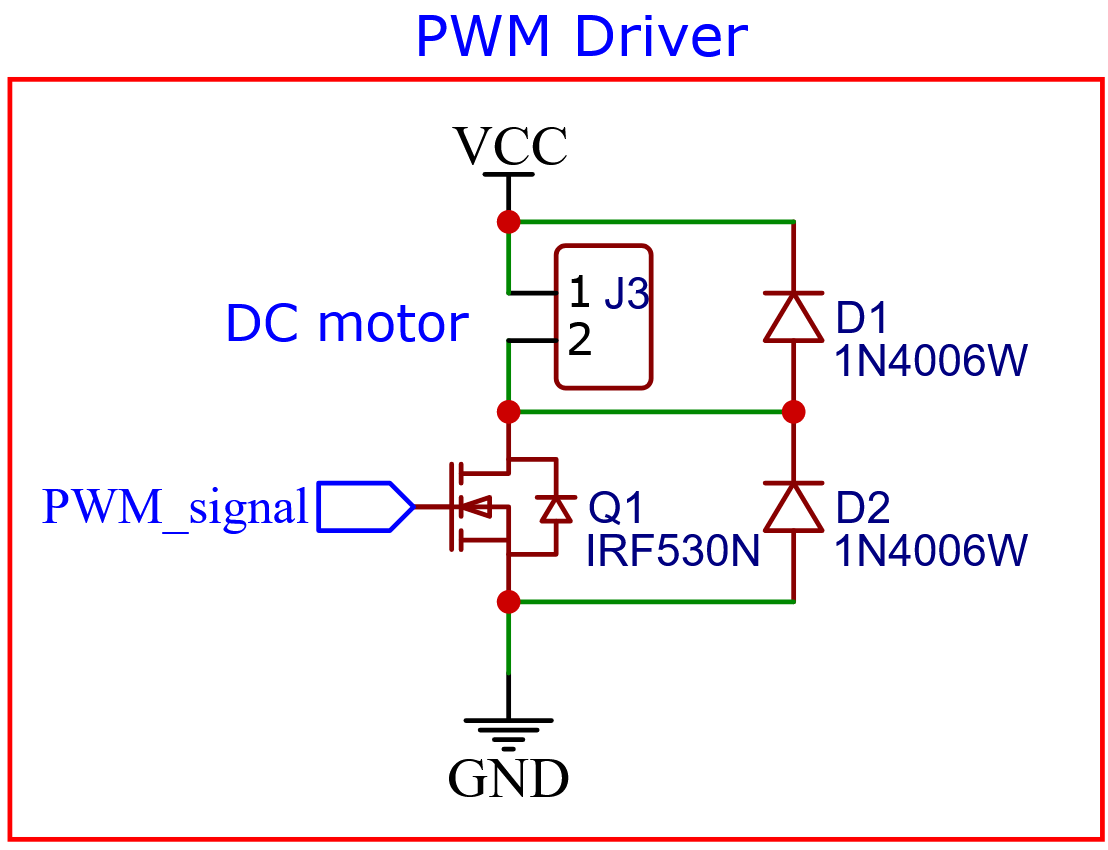
\includegraphics[width=\textwidth]{Dokumentation/Figures/PWM_Driver.png}
     \caption{PWM Driver Schematic}
     \label{fig: PWM Driver Schematic}
     \end{figure}


\section{Test}
Følgende kravspecifikationer tilhører denne del af projektet
\begin{enumerate}
  \item V1 skal være 15V +/- 1 volt for en buck strøm på 100 mA
  \item AC-generator systemet skal kunne levere 300 mA til buck konverteren.
  \item Ved en belastningsændring fra 100mA til 300 mA skal V1 overholde krav 1, indenfor 1.0 s.
\end{enumerate}

For at teste Krav 1, belaster vi udgangen af buck konverteren (4.8V) med 16$\Omega$ hvilket svarer til nogenlunde 100mA ved 15V. Det kan ses på Figur \ref{fig: Krav 1 Opfyldt} at spændingen er 14.9V, og kravet dermed er overholdt.
\begin{figure}[H]
      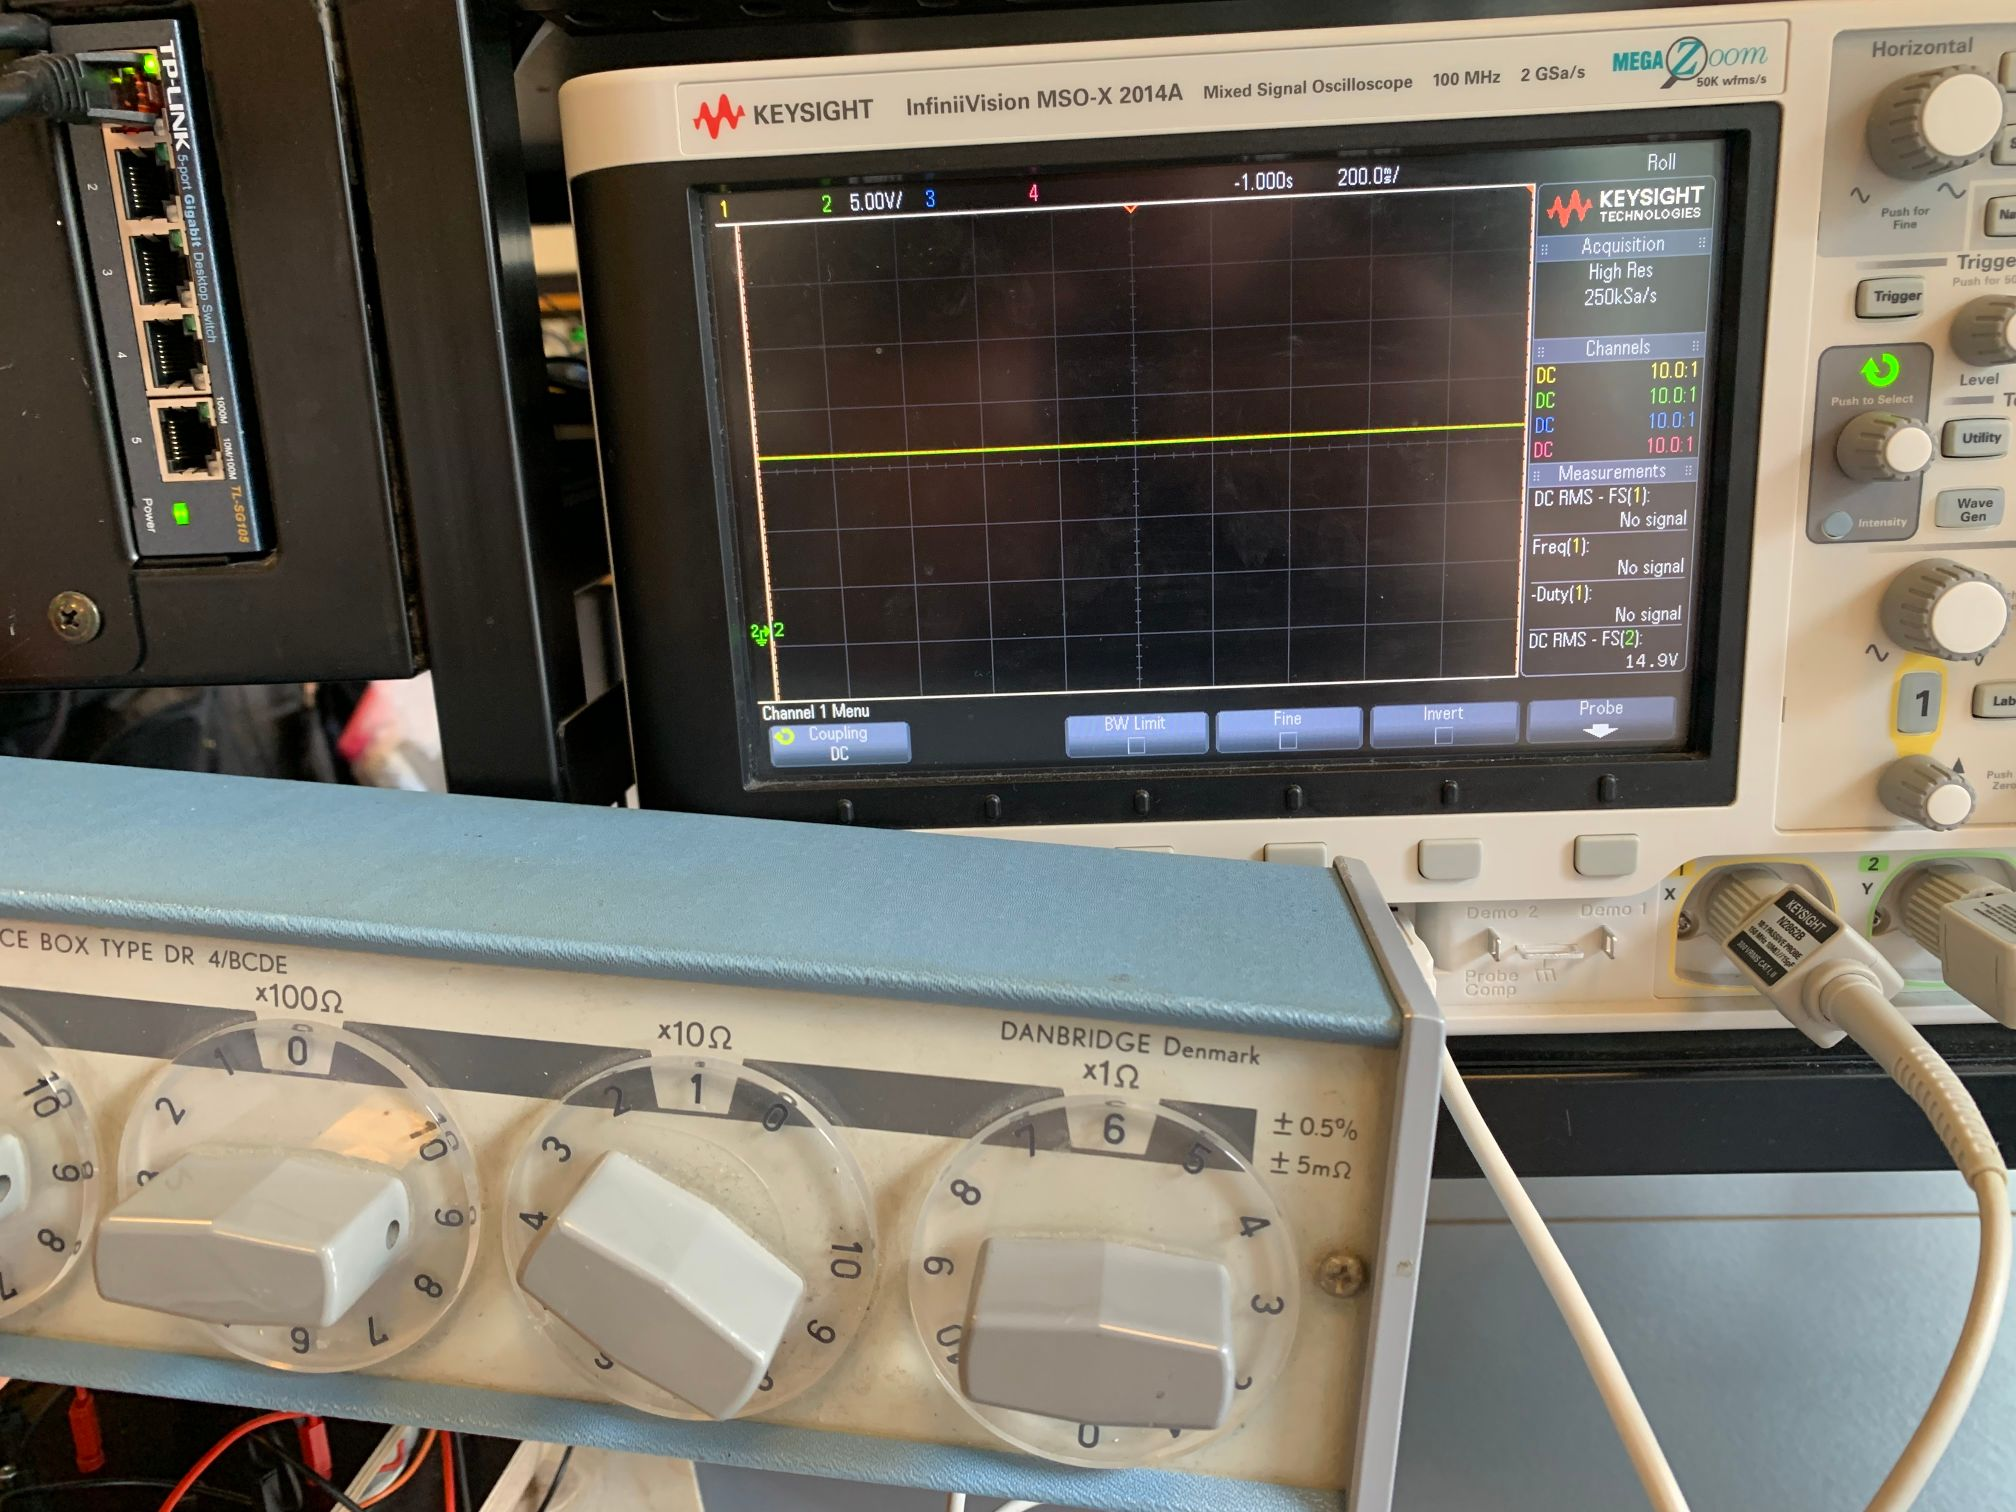
\includegraphics[width=\textwidth]{Dokumentation/Pictures/Krav1.jpg}
     \caption{Krav 1 Opfyldt}
     \label{fig: Krav 1 Opfyldt}
     \end{figure}

For at teste Krav 2, belaster vi udgangen af buck konverteren (4.8V) med 5$\Omega$ hvilket svarer til nogenlunde 300mA ved 15V. Det kan ses på Figur \ref{fig: Krav 2 Opfyldt} at spændingen er 14.9V, og kravet dermed er overholdt.
\begin{figure}[H]
      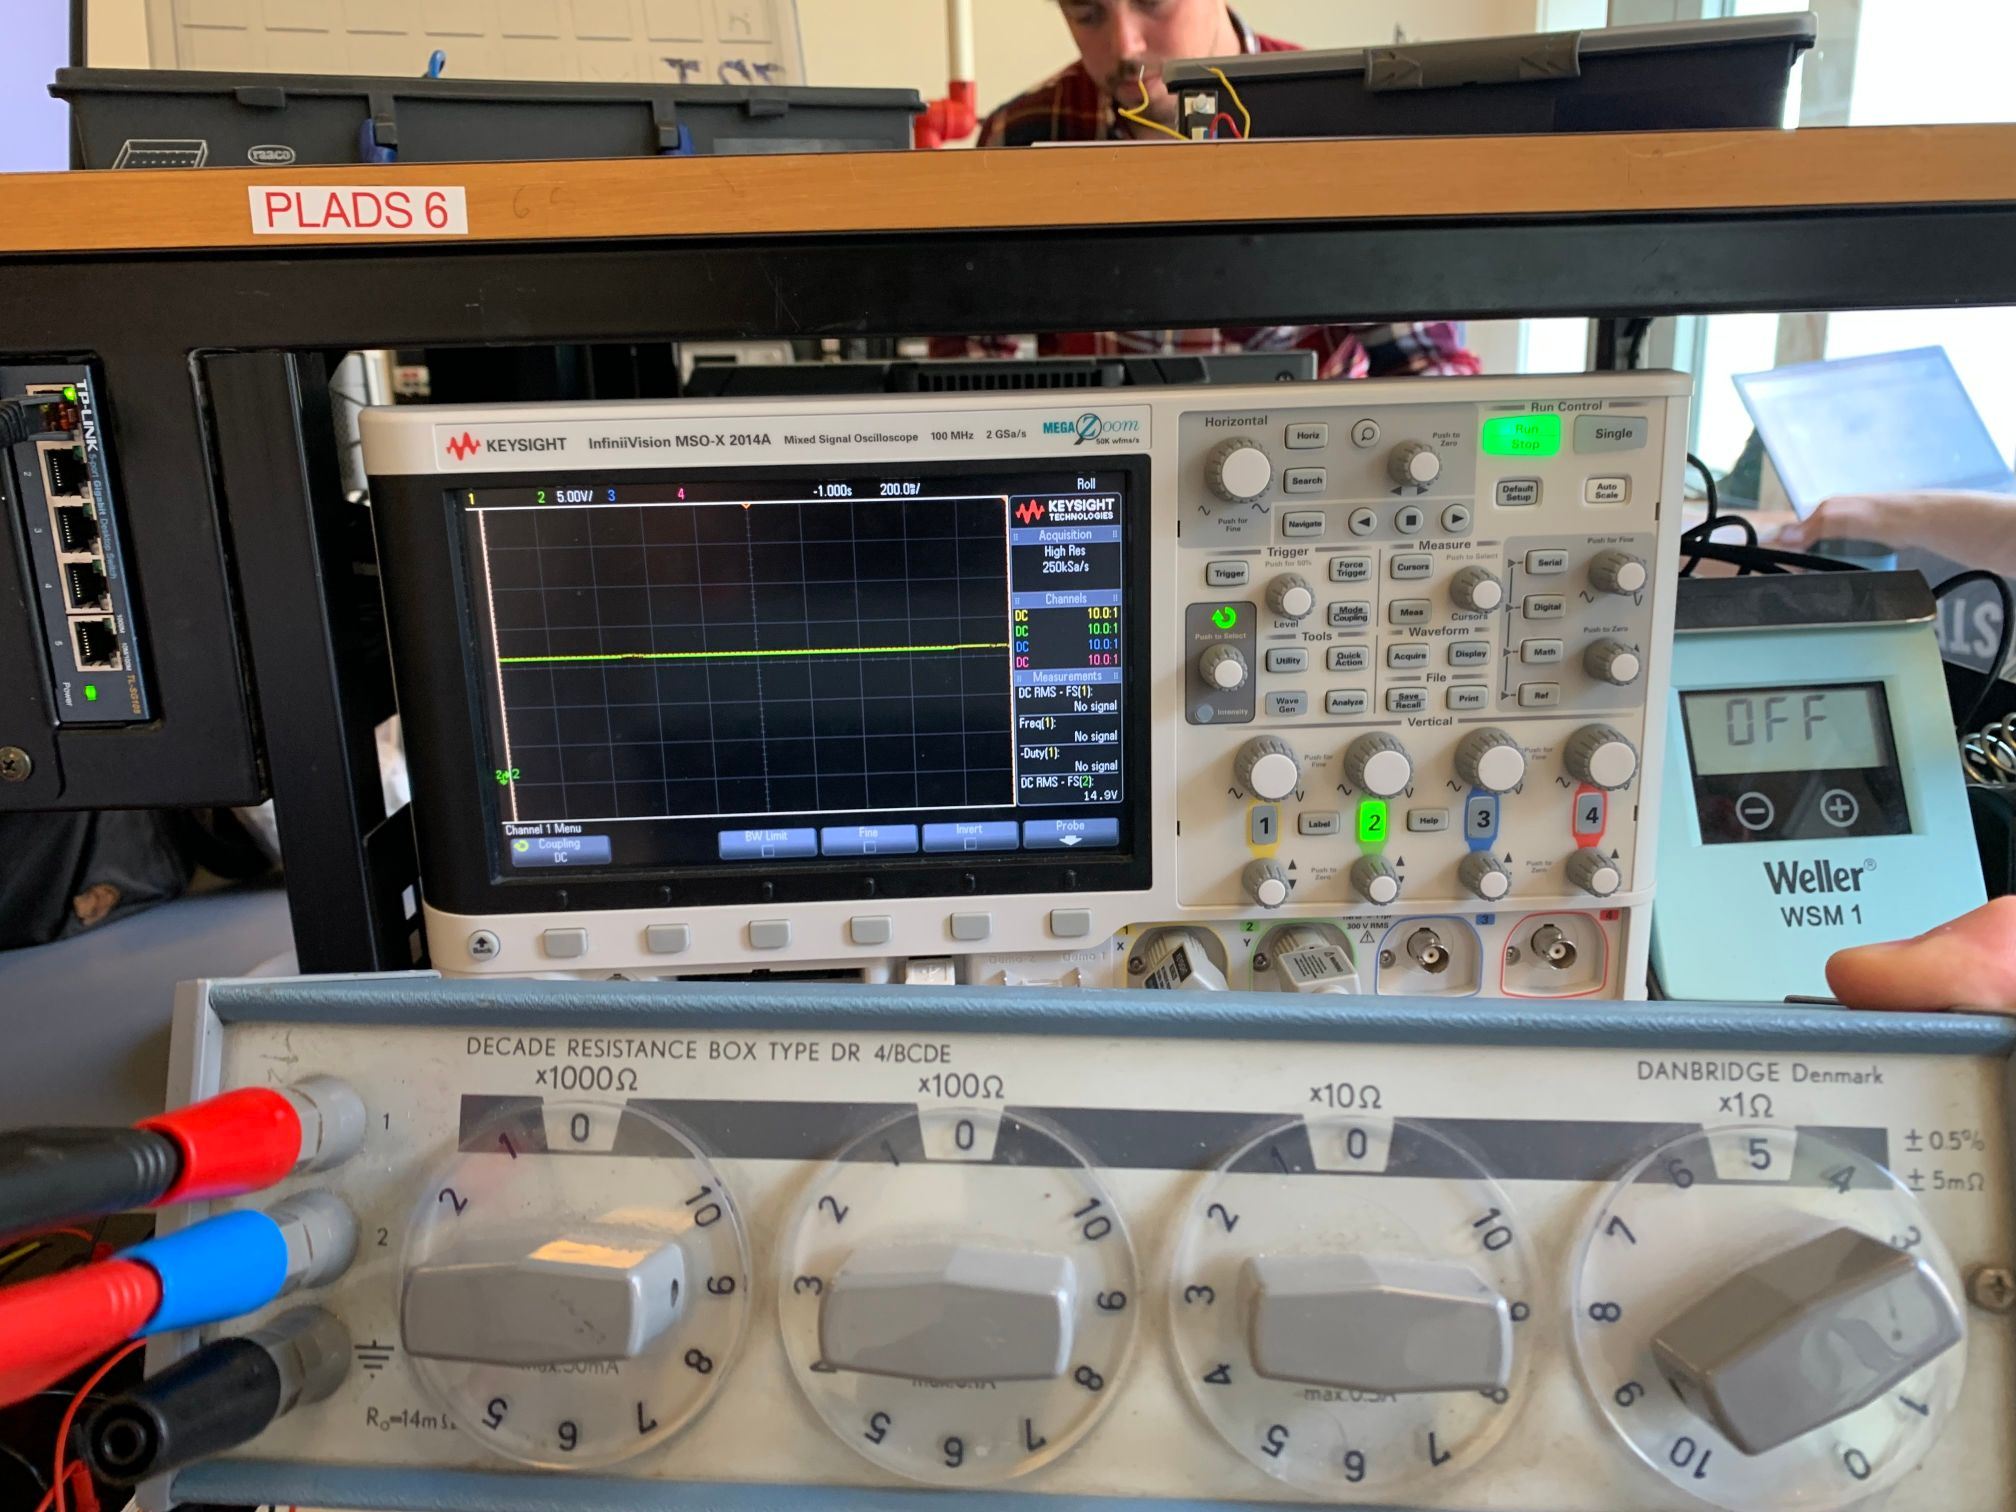
\includegraphics[width=\textwidth]{Dokumentation/Pictures/Krav2.jpg}
     \caption{Krav 2 Opfyldt}
     \label{fig: Krav 2 Opfyldt}
     \end{figure}

For at teste Krav 3, belaster vi udgangen af buck konverteren (4.8V) med 5$\Omega$ og skifter den derefter hurtigt til 164$\Omega$ hvilket svarer til nogenlunde at hoppe fra 100mA til 300mA ved 15V. Det kan ses på Figur \ref{fig: Krav 3 Opfyldt} at spændingen er -1V efter 1 sekund, og kravet dermed er overholdt.
\begin{figure}[H]
      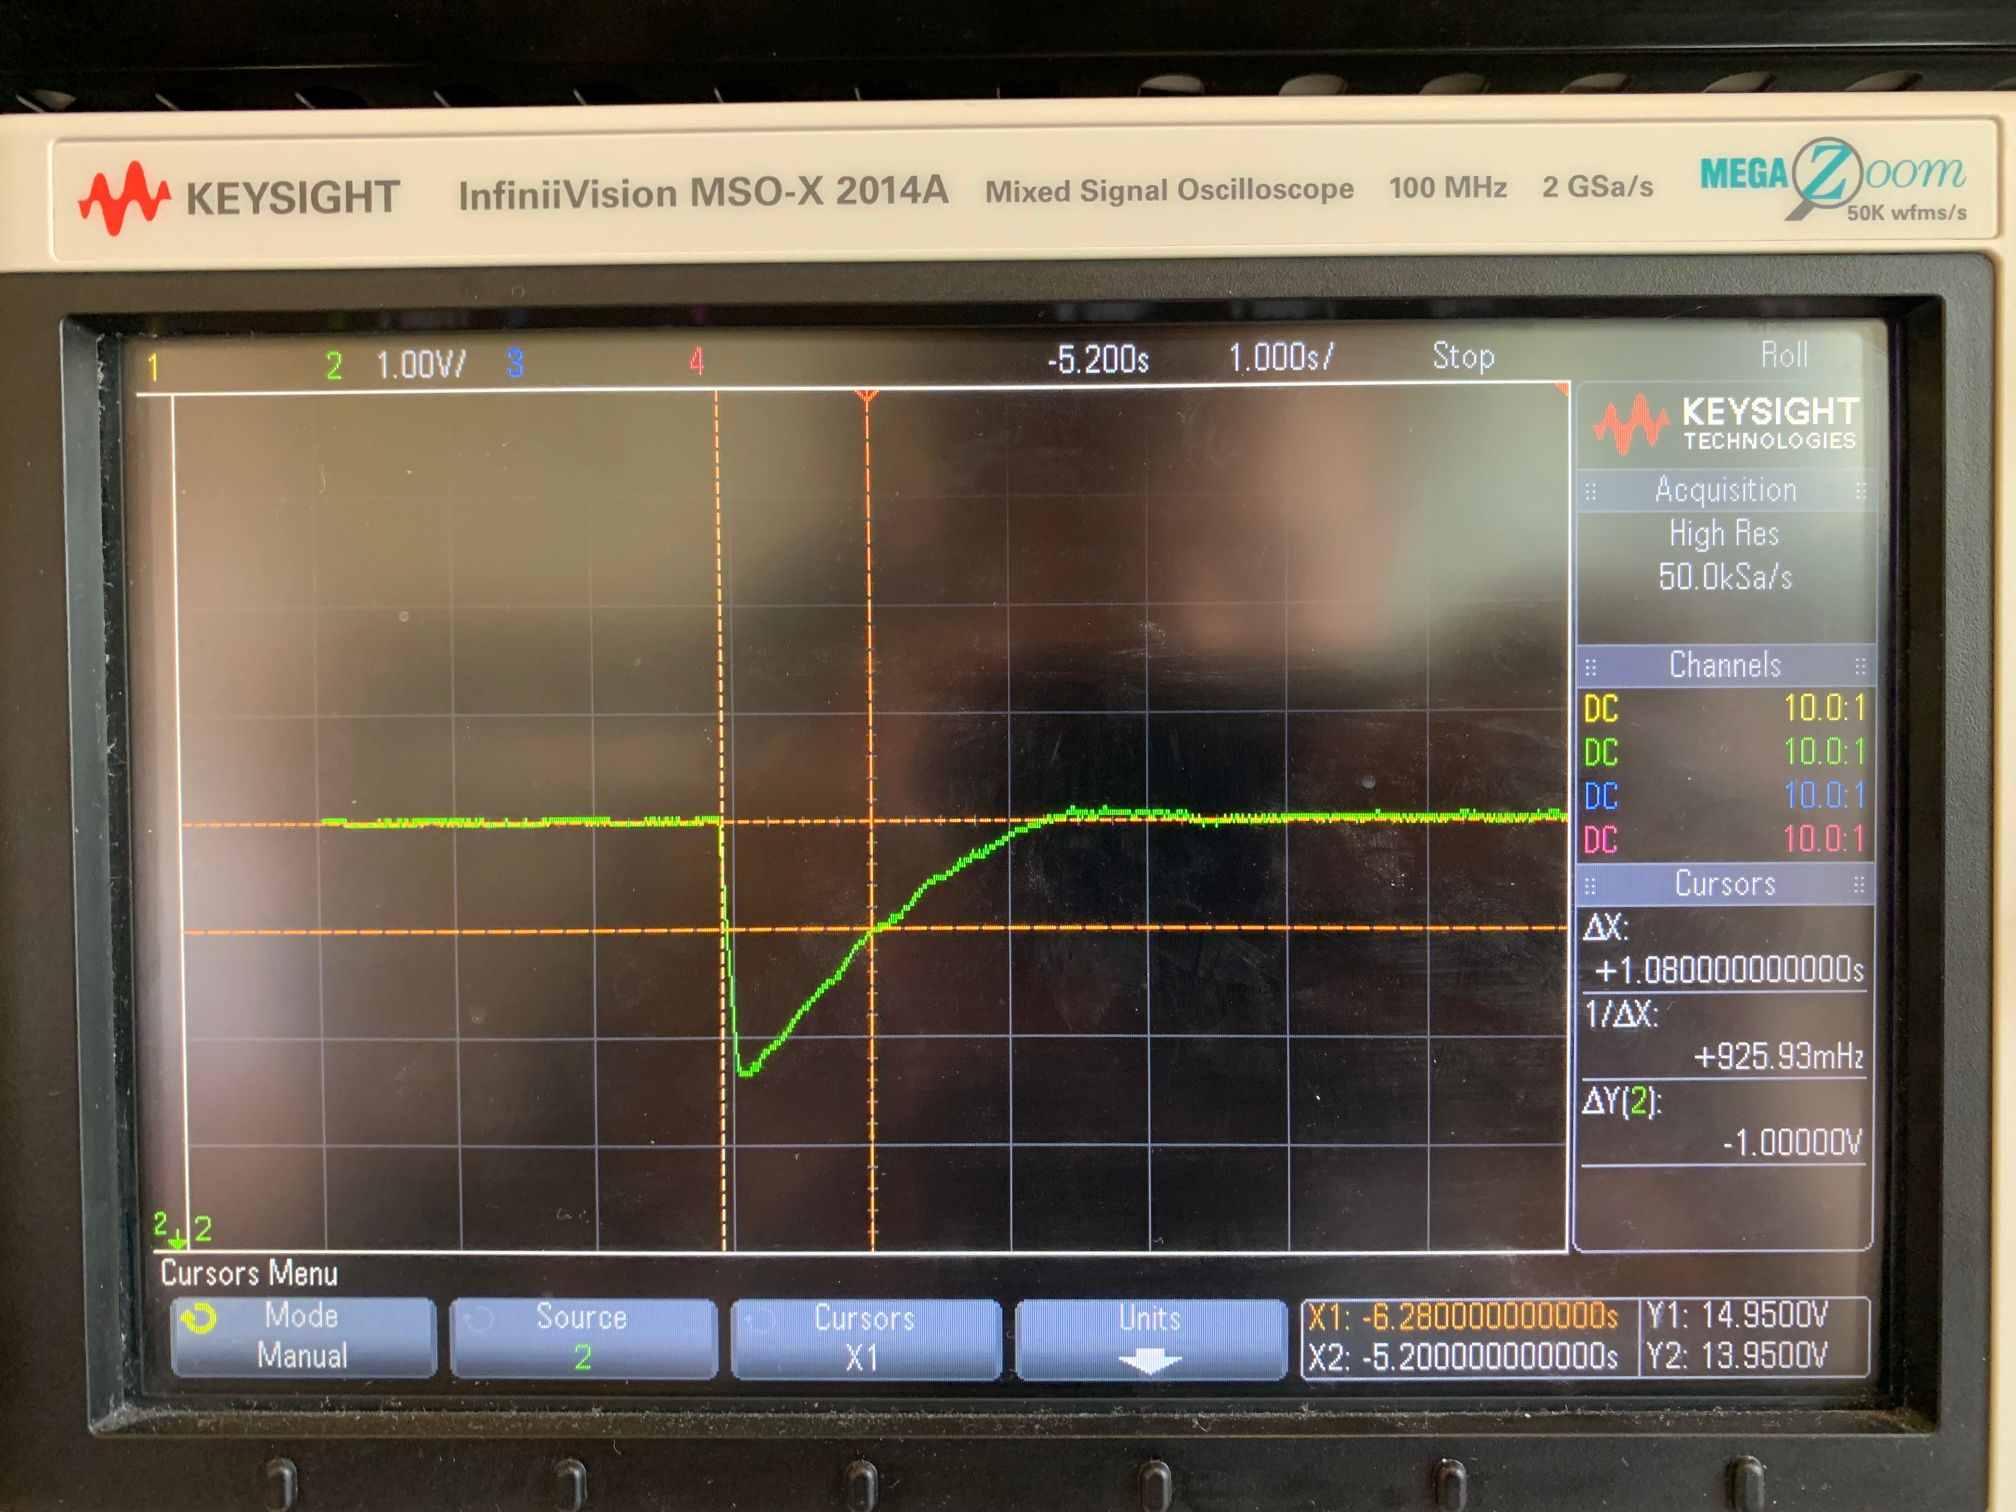
\includegraphics[width=\textwidth]{Dokumentation/Pictures/Krav3.jpg}
     \caption{Krav 3 Opfyldt}
     \label{fig: Krav 3 Opfyldt}
     \end{figure}

De tre krav er allesammen overholdt, og testen er dermed en succes. 

     
\end{document}